\documentclass[a4paper]{article}
% Please do not change with the font size, line height, and the vertical spacing


\usepackage{amssymb}
\usepackage{amsmath} %math environment
\usepackage{algorithm} %pseudo code algorithm
\usepackage{algpseudocode}
\setcounter{tocdepth}{3}
\usepackage{graphicx}
\usepackage{booktabs} % please use booktabs for tables (toprule, midrule, bottomrule)

\usepackage{todonotes}

\PassOptionsToPackage{hyphens}{url}
\usepackage{hyperref}
\usepackage{url}
\usepackage{array}

% using UTF-8 file format allows you to write umlauts into the document
\usepackage[utf8]{inputenc}
\usepackage[T1]{fontenc}

\urlstyle{rm}

\usepackage[protrusion=true,expansion=false]{microtype}

\usepackage{adjustbox}
\usepackage{tikz}
\usetikzlibrary{positioning,arrows,fit,calc}
\pgfdeclarelayer{bg}
\pgfsetlayers{bg,main}
\tikzset{
    >=stealth'
}

\begin{document}
	
% Insert your name and student number (only in the final seminar paper):
% \author{Mary Miller (1231234) \and Richard Pollock (your student number)}
\author{
	Frank Kaiser\\ % Your name
} % leave the author empty for surveys (double-blind review process) 
%\institute{} % the institute should always be left empty


% the title of your topic in title case (special capitalization rules apply, see comment below)
\title{Test Cost Estimation of Model-based Embedded Software} 

% Capitalization rules taken from http://static.springer.com/sgw/documents/1121537/application/pdf/SPLNPROC+Author+Instructions_Feb2015.pdf:
% Headings should be capitalized (i.e., nouns, verbs, and all other words except articles, prepositions, and conjunctions should be set with an initial capital) [...] Words joined by a hyphen are subject to a special rule. If the first word can stand alone, the second word should be capitalized. Here are some examples of headings: “Criteria to Disprove Context-Freeness of Collage Languages”, “On Correcting the Intrusion of Tracing Non-deterministic Pro- grams by Software”, “A User-Friendly and Extendable Data Distribution System”, “Multi-flip Networks: Parallelizing GenSAT”, “Self-determinations of Man”.

%\setlength{\parindent}{0pt}

\newcommand{\tikzimg}[3]{
    \begin{figure}[h!]
        \centering
        \begin{adjustbox}{max width = \textwidth}
            \input{#1}
        \end{adjustbox}
        \caption{#2}
        \label{#3}
    \end{figure}
}

\makeatletter
\begin{titlepage}
    
    \newcommand{\HRule}{\rule{\linewidth}{0.5mm}} % Defines a new command for the horizontal lines, change thickness here

\center % Center everything on the page
 
%----------------------------------------------------------------------------------------
%	HEADING SECTIONS
%----------------------------------------------------------------------------------------

\Large{Otto-Friedrich University Bamberg}\\[0.5cm]  % Name of your university/college


\includegraphics[width=3.5cm]{logo.png} % Include a department/university logo - this will require the graphicx package 
\\[0.0cm]

\LARGE{Lehrstuhl für Softwaretechnik und Programmiersprachen}\\[0.5cm] % Major heading such as course name
\vspace{1cm}
\LARGE{Bachelor's Thesis}\\[0.5cm]
\large{Im Studiengang Software Systems Science}\\
\large{der Fakultät Wirtschaftsinformatik und Angewandte Informatik}\\
\large{der Otto-Friedrich Universität Bamberg}\\
\vspace{1.5cm}
\large{Zum Thema}\\[0.5cm] % Minor heading such as course title

%----------------------------------------------------------------------------------------
%	TITLE SECTION
%----------------------------------------------------------------------------------------

%\HRule \\[0.4cm]
{\huge Test Cost Estimation of}\\[0.2cm]
{\huge Model-based Embedded Software}\\[0.4cm] % Title of your document
%\HRule \\[1.5cm]
 
 \vspace{2cm}
 
%----------------------------------------------------------------------------------------
%	AUTHOR SECTION
%----------------------------------------------------------------------------------------

\large{Vorgelegt von:}\\[0.0cm]
\LARGE{Frank Kaiser}\\[0.3cm]

\large{Themensteller:}\\
\large{Prof. Dr. Gerald Lüttgen}\\[0.3cm]

% If you don't want a supervisor, uncomment the two lines below and remove the section above
%\Large \emph{Author:}\\
%John \textsc{Smith}\\[3cm] % Your name

%----------------------------------------------------------------------------------------
%	DATE SECTION
%----------------------------------------------------------------------------------------
\large{Abgabedatum:}\\
{\large \today}\\[2cm] % Date, change the \today to a set date if you want to be precise

%----------------------------------------------------------------------------------------
%	LOGO SECTION
%----------------------------------------------------------------------------------------


 
%----------------------------------------------------------------------------------------

\vfill % Fill the rest of the page with whitespace

\end{titlepage}

%\thispagestyle{empty}
\pagenumbering{Roman}
\tableofcontents
\clearpage
\listoffigures
\clearpage




% Sections are not necessary for literature surveys
% \section{Introduction}
% \label{sec:Introduction}

% Please avoid \\, use paragraphs (two newlines instead)
% Please avoid texttt (use \emph instead)
% You can include figures in your survey (mostly not appropriate). Please use floats for that purpose and reference all figures.
% Please do not start sentences with a \cite; use the name of the author or the first author et al. instead.
% Please check your spelling, punctuation, and typography. For instance, use -- for dashes like this: This finding was -- according to the authors -- a significant finding.
% Please use appropriate quotation marks if you cite text verbatim (mostly rephrasing is better). In LaTeX quoatation marks are not printed with " but as follows: ``text''

% Start your survey here
\pagenumbering{arabic}
\setcounter{page}{1}

\begin{abstract}
In this paper, we analyze the different ways to disclose software vulnerabilities. Based on our reviewed literature, we found that the hybrid disclosure method is most often the preferred one as it benefits society and software vendors the most, as it's goal is to combine the advantages of other disclosure policies. Additionally we present a short overview on how to disclose a vulnerability based on the CERT/CC disclosure guide. We then continue to show differences in patch behavior between open source and proprietary software vendors and show the risks and incentives when disclosing vulnerabilities. Finally, we give examples of recent vulnerabilities and their disclosures and analyze them according to the findings of this paper.
\end{abstract}

\section{Introduction}

The word vulnerability origins from the Latin word vulnus, or ``wound''. If a human is wounded, it is quite obvious to see a doctor, but if a computer is wounded, nobody might even notice. Therefore, whenever someone encounters a ``wound'', they should disclose it to the corresponding authorities to provide a patch. Similar to our health care system, where many parties need to work together to ensure the patient's health, it is important that software vendors cooperate with researchers, academics, penetration testers or any user of their product to improve their software's security.

%Everyday more and more software based devices are built and distributed in our environment. While they provide useful services or are just very convenient, every one could contain a flaw, allowing adversaries to break into such devices and steal valuable, private information. Therefore it is of greatest importance that software vendors work together with researchers, academics, penetration testers or any user of their product to improve its software security. Since computers became dominant in our lives, different ways to disclose vulnerabilities have emerged. 

In this paper we introduce three different types of disclosure (\autoref{sec:types_disclosure}) after we establish the terminology in \autoref{sec:vuln_background}. In \autoref{sec:guide} we present a guide for coordinated vulnerability disclosure from the perspective of the discoverer of the vulnerability. We proceed with a short comparison between open source and closed source software vendors in terms of disclosure (\autoref{sec:open_vs_prop}) and provide several incentives and risks for disclosure in \autoref{sec:risks_incentives}. Lastly we give some examples of vulnerability disclosure happened in recent times in \autoref{sec:examples}.


%\vspace{50pt}
%\todo{possible quotes for intro?}

%"Vulnerability disclosure is a process through which vendors and vulnerability finders may work
%cooperatively in finding solutions that reduce the risks associated with a vulnerability. It encompasses
%actions such as reporting, coordinating, and publishing information about a vulnerability and its
%resolution." \cite{ISO29147:2014}

%\vspace{50pt}

%Reports that say that something hasn’t happened are always interesting to me, because as we know, there are known knowns; there are things we know we know. We also know there are known unknowns; that is to say we know there are some things we do not know. But there are also unknown unknowns – the ones we don’t know we don’t know. – Donald Rumsfeld

% What is Vulnerability / Bug? Lifecycle Schryen 2011


\section{Background}\label{sec:vuln_background}

This section establishes the terminology used in this paper and gives an
overview of the terminology used in other works.

\subsection{Glossary}

This section briefly explains terms used in the SIBAS G programming language.

\paragraph{Program} The complete SIBAS program that can be compiled and uploaded to run cyclical on its device. It is hierarchic ordered into function packages.

\paragraph{Function Package} A function package describes a broader functionality of a component, e.g. the parking brake, and consists of multiple function groups.

\paragraph{Function Group} Function groups are the smallest part of the program hierarchy. They can either contain multiple function groups or models describing the software. The model itself consists of two entities: function blocks and signals.

\paragraph{Function Block} Function blocks are predefined methods that can take multiple inputs and have multiple outputs.

\paragraph{Signal} The variables of the program are projected as signals. Visually they are either represented by a flag when they don't origin in the current function group or otherwise as a line between two function blocks.

\paragraph{Function ID} Function IDs are unique identifiers that are assigned by the developer to function groups that implement a common function. A function ID consists of at least one function group, though more complex functions are spread over multiple IDs.

\subsection{SIBAS Control Technology}

SIBAS 32, the successor of SIBAS 16, is a control technology used in trains. Its goal is to provide a common interface between different components, e.g. central control device or brake control device. SIBAS 16 was first introduced in 1983 and was further developed until in 1992 SIBAS 32 was released. The software that runs SIBAS is projected in an editor called SIBAS G in a model-based approach. The model translates automatically into C code and eventually compiles to run as intended on embedded systems. Every function block is validated before being allowed to use, hence when testing the software, only the logic of the software needs to be tested.


\subsection{SAMAPI - Sibas Application Model API Specification}

SAMAPI provides the possibility to read or create SIBAS models.
It is written in Java but is distributed to use in Python 2.7 via Jython\footnote{\url{http://www.jython.org/docs/index.html}}.

\begin{figure}[ht]
	\centering
	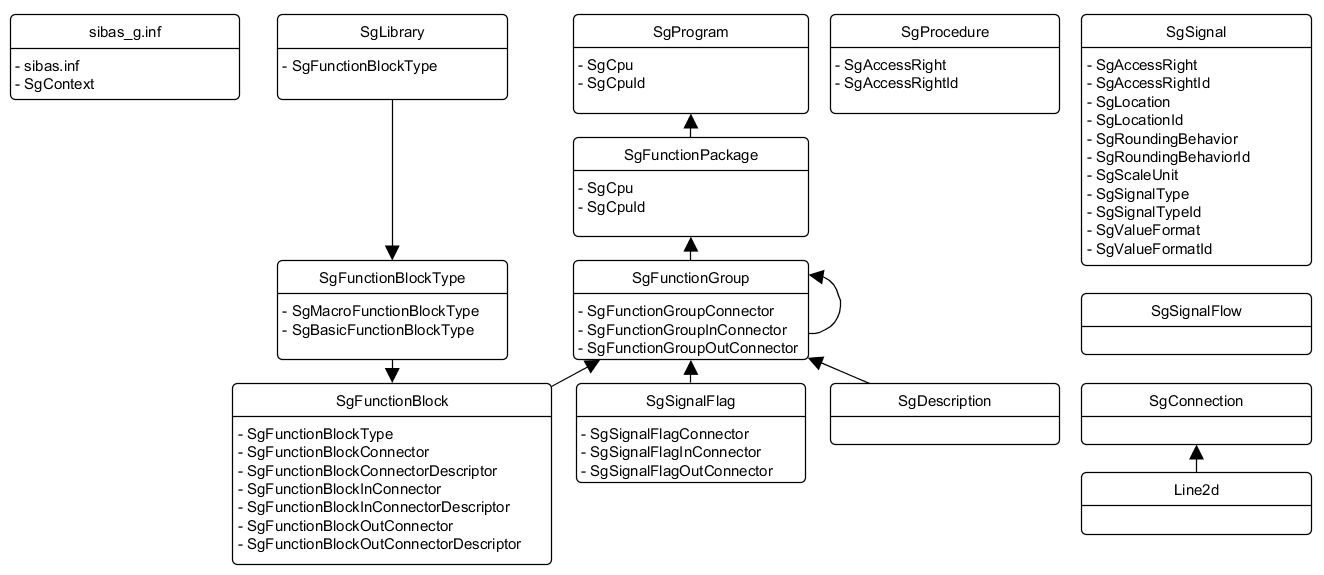
\includegraphics[width=1\textwidth]{graphic/samapi_classes.png}
	\caption{SAMAPI - Class Overview}
	\label{fig:samapi}
\end{figure}

\autoref{fig:samapi} describes the structure of the API.









\section{Approach}

In this section the general approach is described.

\subsection{Halstead-Metric} \label{sec:background:halstead}

As described in section \autoref{background:halstead} the relevant parameters are operands and operators.
However, for model-based software it is not as obvious

\subsection{Cyclomatic-Complexity}

Parameterwahl etc.

\subsection{Halstead Metric} 

\section{Evaluation}\label{sec:eval}

In order to evaluate these approaches, the resulting values are normalized to a scale from zero to ten (Equation \ref{math:normalize}, though zero is only the result if the value could not be computed, e.g. when resulting parameters would divide by zero. Additionally, test engineers were conducted and rated different projects using the same scale. Eventually, the euclidean distance (see \autoref{math:euclid_distance})  is used to calculate the distance of each data set in regard to the manually conducted approach.

\begin{equation}
\label{math:normalize}
X^{'} = \frac{X - X_{min}}{X_{max} - X_{min}} * 10
\end{equation}

\begin{equation} 
	\label{math:euclid_distance}
	d(p,q) = \sqrt{\displaystyle\sum_{i=1}^{n} (p_i - q_i)^2}
\end{equation}
	
In total, ten function packages of three projects were evaluated by three different experts. For function IDs, the results for the euclidean distance of each approach to the experts estimation can be seen in \autoref{fig:euclid_distance_fid_result}. For the approach by function groups \autoref{fig:fg_result} shows the results.
The values marked red are the lowest and therefore the closest to the experts reference, while green marks the biggest number, which indicates a large difference in values. For both testing methods (function ID and function group) the Halstead difficulty is performing best with having the smallest euclidean distance in 17 of 20 cases. Cyclomatic complexity showed to be right in the middle between the signal depth analysis (SDA) and the Halstead difficulty.

\begin{figure}[ht]
	\centering
	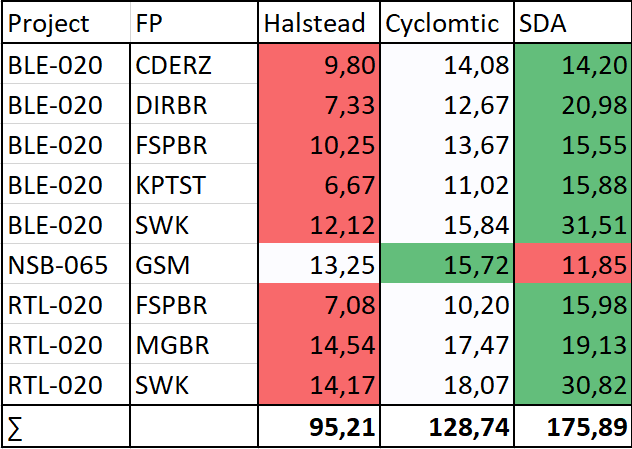
\includegraphics[width=0.7\textwidth]{graphic/FID_RESULT.png}
	\caption{Euclidean distance - Function ID approach} 
	\label{fig:euclid_distance_fid_result}
\end{figure}

\begin{figure}[ht] 
	\centering
	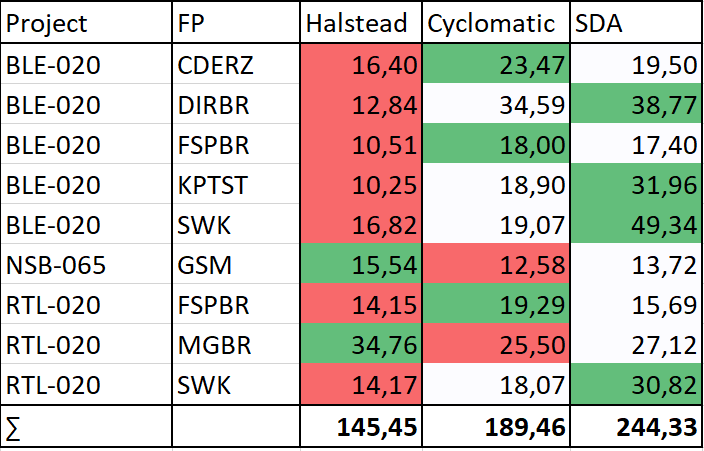
\includegraphics[width=0.7\textwidth]{graphic/FG_RESULT.png}
	\caption{Euclidean distance - Function Group approach}
	\label{fig:fg_result}
\end{figure}

In one case SDA performed best in the function ID approach. In \autoref{fig:plot_gsm_fid} the three examined approaches and the expert evaluation are plotted for NSB 065 - GSM. Function ID 4 is one of the few cases, where the experts evaluation is higher than all approaches. Though when studying all data sets, SDA scores usually the highest overall. This may be one of the reasons, why SDA performed worst in most cases, as the experts rated mostly between two and six. Though all approaches seem to have similar tendencies, since the plots changes mostly in the same directions. It seems the biggest difference between all approaches is the scale. General more complex function packages may be better analyzed by SDA, while more common ones using Halstead.

\begin{figure}[ht]
	\centering
	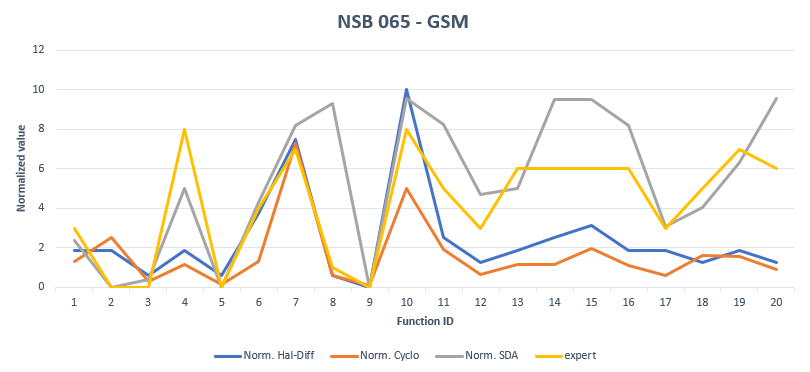
\includegraphics[width=1\textwidth]{graphic/NSB-GSM_plot.png}
	\caption{Complexity comparison NSB - Function ID approach}
	\label{fig:plot_gsm_fid}	
\end{figure}

\begin{figure}[ht] 	
	\centering
	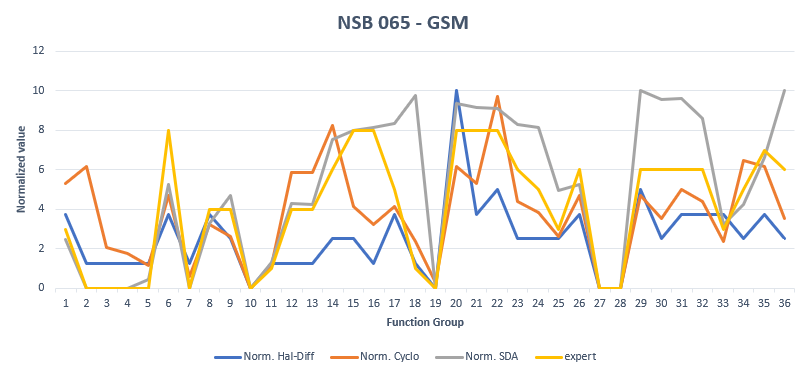
\includegraphics[width=1\textwidth]{graphic/NSB-GSM_FG_plot.png}
	\caption{Complexity comparison NSB - Function Group approach}
	\label{fig:plot_gsm_fg}
\end{figure}

\begin{figure}[ht]
	\centering
	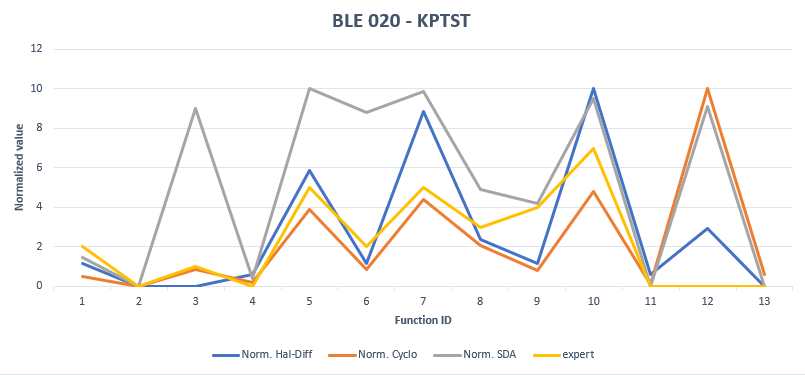
\includegraphics[width=1\textwidth]{graphic/BLE-KPTST_plot.png}	
	\caption{Complexity comparison BLE - Function ID approach}
	\label{fig:plot_ble_fid}
\end{figure}

\begin{figure}[ht]	
	\centering
	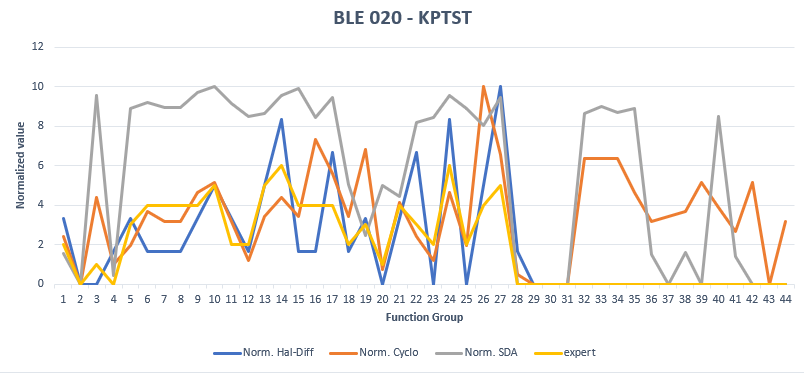
\includegraphics[width=1\textwidth]{graphic/BLE-KPTST_FG_plot.png}
	\caption{Complexity comparison BLE - Function Group approach}
	\label{fig:plot_ble_fg}
\end{figure}

%\section{Open Source vs Proprietary Vendors}
\label{sec:open_vs_prop}
In this section we highlight the difference of disclosing vulnerabilities to open source or proprietary vendors.

\subsection{Patch Release Time}

There is an ongoing debate whether open-source software is really faster at providing patches than proprietary vendors. Arora et. al conducted an empirical study and randomly chose 131 vulnerabilities published by CERT or SecurityFocus or both and conclude that open source vendors do release patches quicker than closed source vendors \cite{Arora10_Patch_Release}. Schryen, however, chose 17 open source and closed source packages with roughly the same functionality and found that there is no meaningful difference in patching behavior \cite{Schryen2011}. Though one could argue that Schryen's findings are less significant due to a limited number of samples.

\subsection{Disclosing Vulnerabilities in Open Source Software}

``There is no security through obscurity'' is a common mantra in open source software, suggesting that open source vendors don't fear a vulnerability disclosure, but rather welcome one. Though according to Swire there are some cases, where secrecy is preferred, because a potential attacker would get more relevant information, such as passwords and secret keys used for authorization, than the defender \cite{Swire06TheoryOfDisclosure}.

Additionally intrusion detection systems used to detect attackers, especially in the form of so called ``honeypot'' (a trap in a system made to lure attackers), can lose their effectiveness when bad actors know of their existence.
Lastly Swire mentions secrecy in nonstandard configurations and settings when using open source software. For example SSL is a protocol that provides secure communication among multiple parties. By tweaking it, it is achievable that only machines that know the tweak are able to communicate with each other.

\subsection{Disclosing Vulnerabilities in Proprietary Software}

For vendors of proprietary software there is always an incentive to keep disclosure out of the public, as open vulnerabilities could harm their sales, though if such information gets public afterwards the image of the vendor could be damaged long-term. Hence most vendors are very likely to take part in responsible disclosure \cite{Swire06TheoryOfDisclosure}.

\section{Related Work}


\subsection{Empirical Study of Software Metrics}

In 1987 Li and CHEUNG published their empirical study of software metrics \cite{LI:1987-Study-of-Software-Metrics}. They wrote a static Fortran source code analyzer to automatically analyze 255 different programs (student assignments) and compared 31 different metrics including a new introduced metric. They divide these static measures in three categories: Volume, measuring the size of a product, Data Organization, measuring usage and visibility of data, and Control Organization, measuring the comprehensibility of control structures. Halstead metrics would be in the first category, while McCabe's cyclomatic complexity fits the second one. LI and Cheng propose to first use Halstead metrics to put the analyzed software in different categories and then use cyclomatic complexity to a more fine-grained estimation in each category. He concludes that the validity of any tested measure cannot be asserted with precision and that a metric is valid if it succeeds to reflect what it it meant to measure.

\subsection{Calculation and Visualization of Model Complexity in Model-based, Safety-relevant Software}

Stürmer et al. estimate complexity of model-based software by applying the Halstead metrics on a model \cite{Stuermer:2010}. They argue against cyclomatic complexity in their usecase as the model complexity is not significantly affected by control flow, but by the amount of blocks and how they are connected with their corresponding signals. As parameters used for the Halstead metrics they chose mostly similar values as shown here in \autoref{sec:approach-halstead}, though for \(N_2\) they decided to choose the amount of outgoing signals for a function block.



%\vspace{3cm}
%Neural Network
%https://ascelibrary.org/doi/abs/10.1061/(ASCE)0733-9364(1998)124:3(210)


%An Assessment and Comparison of Common Software Cost
%Estimation Modeling Techniques
%https://dl.acm.org/citation.cfm?id=302647
%http://www.ehealthinformation.ca/wp-content/uploads/2014/07/isern-98-27.pdf



\section{Future Work}

\subsection{Integrating into Toolchain}

The sbtSWAT functionality shall be integrated into the current tool in use that allows test automation.

\subsection{Time Cost Estimation}

One of the reasons the test cost of software is established, is to help planning the test order. If a reasonable time frame can be derived without having to examing the software, project planners will have a easier time meeting the deadline to a software release. In order to achieve a good time estimation, the time needed for every function group needs to be noted and put in relation to the estimated complexity values.

\section{Conclusion}

Fog is here. And it is here to stay. Fog is just at its start and as the cloud grew over the last 20 years, fog will follow suit and change over the course of its lifespan. Though the basic mantra to let computation, storage and control occur closer to the end user will stay until new drastic technical progress will be made.


\section{Acknowledgement}


% This template uses bibtex for the bibliography. You can also use biblatex.

% Please include *complete* references (copy&paste the whole bibtex entries, i.e., for the paper as well as the cross-referenced conference as provided by dblp whenever possible)
% These bibtex entries may need some further editing to make them homogenuous)

\clearpage
\bibliography{literature}
\bibliographystyle{splncs03}

\newpage

\textbf{Eingeständigkeitserklärung}
\vspace{2cm}

Ich erkläre hiermit gemäß §17 Abs. 2 APO, dass ich die vorstehende Bachelorarbeit
selbstständig verfasst und keine anderen als die angegebenen Quellen und Hilfsmittel
verwendet habe.

\vspace{2cm}

Bamberg, den 11. Oktober, 2018 \hspace{3cm} Frank Kaiser
\end{document}




